\chapter{La gerarchia polinomiale} \label{ch:capitolo15}
\subsection{NP e coNP}
\textbf{Definizione}\\
Ricordiamo che coP è la classe dei problemi il cui complemento appartiene
alla classe P. 
\\Poniamo:
\begin{figure}[htp]
    \centering
    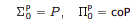
\includegraphics[scale=0.9]{tesi_stile/img/figura1cap15.png}
\end{figure}
\\\\Come già osservato,\\
\begin{figure}[htp]
    \centering
    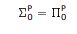
\includegraphics[scale=0.9]{tesi_stile/img/foto2cap15.png}
\end{figure}
\\\textbf{Definzione}
\\Poniamo:\\
\begin{figure}[htp]
    \centering
    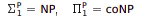
\includegraphics[scale=0.9]{tesi_stile/img/foto3cap15.png}
\end{figure}
\begin{center}
    NP = coNP?
\end{center}
\textbf{Esempio}\\
Come ben noto, SAT $\in$ NP:
\begin{itemize}
    \item Per dimostrare che un sistema di clausole è soddisfacibile, basta esibire una clausola che lo soddisfa (e la lunghezza di tale clausola è polinomialmente limitata dalla dimensione del sistema)
    
    \item Per dimostrare che un sistema di clausole è insoddisfacibile, è necessario verificare che tutte le clausole non soddisfano il sistema (e il numero di tali clausole può essere esponenziale rispetto alla dimensione del sistema)
\end{itemize}
\begin{center}
    UNSAT $\in$ NP ?
\end{center}
\textbf{Definizione}\\
Sia S un problema sull’alfabeto A.
Si ha S $\in$ NP se esistono un problema T $\in$ P e un polinomio $p_s$ tali che per ogni input w
\begin{center}
    $w \in S \Longleftrightarrow \exists y \in A*$ t.c. $l(y) <= p_s (l(w)), (w, y) \in T$
\end{center}
Si ha S $\in$ coNP se esistono un problema T $\in$ P e un polinomio $p_s$ tali che per ogni input w
\begin{center}
     $w \in S \Longleftrightarrow \exists y \in A*$ t.c. $l(y) <= p_s (l(w)), (w, y) \in T$
\end{center}
\textbf{Osservazione}\\
\begin{itemize}
    \item P = coP $\subseteq$ coNP
    
    \item se P = NP, allora coNP = coP = P = NP.
\end{itemize}
\newpage
\begin{figure}[htp]
    \centering
    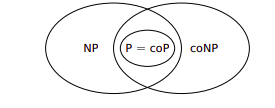
\includegraphics[scale=0.9]{tesi_stile/img/foto6cap15.png}
\end{figure}
\textbf{Definizione}\\
Sia S un problema sull’alfabeto A.\\
Si ha S $\in$ $\sum_{1}^p$ se esistono un problema T $\in$ $\prod_{0}^{P}$ e un polinomio $p_s$ tali che per ogni input w
\begin{center}
      $w \in S \Longleftrightarrow \exists y \in A*$ t.c. $l(y) <= p_s (l(w)), (w, y) \in T$
\end{center}
Si ha S $\in$  $\prod_{1}^{P}$ se esistono un problema T $\in$ $\sum_{0}^p$ e un polinomio $p_s$ tali che per ogni input w
\begin{center}
      $w \in S \Longleftrightarrow \exists y \in A*$ t.c. $l(y) <= p_s (l(w)), (w, y) \in T$
\end{center}
\newpage
\subsection{$\sum_{2}^p$ $\prod_{2}^{P}$}
\textbf{Definizione}\\
Sia S un problema sull’alfabeto A.\\
Si ha S $\in$ $\sum_{2}^p$ se esistono un problema T $\in$ $\prod_{2}^{P}$ e un polinomio $p_s$ tali che per ogni input w
\begin{center}
      $w \in S \Longleftrightarrow \exists y \in A*$ t.c. $l(y) <= p_s (l(w)), (w, y) \in T$
\end{center}
Si ha S $\in$  $\prod_{2}^{P}$ se esistono un problema T $\in$ $\sum_{1}^p$ e un polinomio $p_s$ tali che per ogni input w
\begin{center}
    \begin{figure}[htp]
        \centering
        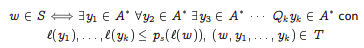
\includegraphics[scale=0.9]{tesi_stile/img/foto7cap15.png}
    \end{figure}
\end{center}
\newpage
\subsection{$\sum_{k}^p$ $\prod_{k}^{P}$}
Sia S un problema sull’alfabeto A e $k >= 1$. Si ha S $\in$ $\sum_{k}^p$  se esistono un problema T $\in$ $\prod_{p}^{k-1}$e un polinomio $p_s$ tali che per ogni input w
\begin{center}
    \begin{figure}[htp]
        \centering
        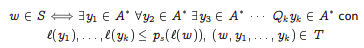
\includegraphics[scale=0.9]{tesi_stile/img/foto7cap15.png}
    \end{figure}
\end{center}
\subsection{Osservazioni}
\begin{itemize}
    \item $\prod_{k}^{p}$ = co$\sum_{k}^p$, k $>=$ 0
    
    \item $\sum_{k}^p$ $\subseteq$ $\sum_{k+1}^p$, $\prod_{k+1}^{P}$ k $>=$ 0
    
    \item $\sum_{k}^p$ $\subseteq$ $\sum_{k+1}^p$, $\prod_{k+1}^{P}$ k $>=$ 0
\end{itemize}
Definiamo
\begin{figure}[htp]
    \centering
    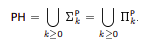
\includegraphics[scale=0.9]{tesi_stile/img/foto8cap15.png}
\end{figure}
\\La sequenza delle classi $\sum_{k}^p$, $\prod_{k}^{P}$, k $>=$ 0 prende il nome di gerarchia polinomiale.
\newpage
\subsection{Gerarchia Polinomiale}
\begin{figure}[htp]
    \centering
    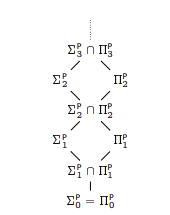
\includegraphics[scale=0.9]{tesi_stile/img/foto9cap15.png}
\end{figure}
\textbf{Proposizione}\\
Si ha PH = P se e solo se P = NP.\\\\
\textbf{Dimostrazione}\\
\begin{itemize}
    \item Supponiamo PH = P. Poichè P $\subseteq$ NP $\subseteq$ PH, si ha P = NP.
    
    \item Viceversa supponiamo P = NP, i.e., $\sum_{0}^p = \sum_{1}^p$. Ne segue
\end{itemize}
\begin{figure}[htp]
    \centering
    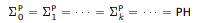
\includegraphics[scale=0.9]{tesi_stile/img/foto10cap15.png}
\end{figure}

e, di conseguenza,  $\sum_{1}^p = \sum_{2}^p$. Iterando,

\begin{figure}[htp]
    \centering
    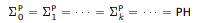
\includegraphics[scale=0.9]{tesi_stile/img/foto10cap15.png}
\end{figure}
\newpage
\textbf{Proposizione}\\
\begin{enumerate}
    \item Se $\sum_{k}^p = \prod_{k}^p$ per qualche k $>= 0$ , allora $\sum_{p}^j = \prod_{p}^j = \sum_{k}^p$ per ogni j $>=$ k. Pertanto, PH = $\sum_{k}^p$.
    
    \item  Se $\sum_{k}^p = \prod_{k}^p$ oppure $\prod_{k}^{p} = \prod_{k+1}^{p}$ per qualche k $>=$ 0, allora $\sum_{p}^j = \prod_{p}^j = \sum_{k}^p$ per ogni j $>=$ k. Pertanto, PH = $\sum_{k}^p$.
    
\end{enumerate}
\textbf{Definizione}\\
Un problema S si dice $\sum_{k}^p$ arduo se per ogni problema T $\in$ $\sum k$ si ha T $<_p$ S. Un problema si dice  $\sum_{k}^{p}$-completo se è $\sum_{k}^{p}$-arduo e appartiene alla classe $\sum_{k}^{p}$
 \\\\\textbf{Proposizione}\\
Per ogni k $>=$ 0 esistono problemi  $\sum_{k}^{p}$-completi
\subsection{Tempi Esponenziali}
PEXP è la classe dei problemi accettati da una macchina di Turing deterministica con complessità temporale O$(2^n)^k$, per un opportuno intero positivo k.
\\LEXP è la classe dei problemi accettati da una con complessità temporale O($c^n$), per un opportuno intero positivo c.
\\Le classi NPEXP e NLEXP sono definite analogamente, ma utilizzando macchine di Turing non deterministiche.
\begin{figure}[htp]
    \centering
    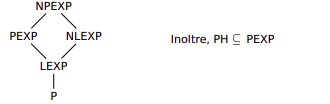
\includegraphics[scale=0.9]{tesi_stile/img/foto11cap15.png}
\end{figure}